% !TeX root = ../jvk-blatt1.tex

\excercise{Einrichtung von IntelliJ}
\label{ex2}

In diesem Kapitel wollen wir dir zeigen wie man IntelliJ einrichtet. IntelliJ ist eine IDE mit der man Java Programme schreiben und ausführen kann. Falls du schon eine andere IDE (z.B. Eclipse) heruntergeladen hast kannst du diese natürlich gerne weiterhin verwenden, unsere Erklärungen werden allerdings von IntelliJ als IDE ausgehen.\newline

\section*{IntelliJ installieren}
\label{ex1}
Gehe zuerst auf die Website \href{\intellijurl}{jetbrains.com/idea/download/} und lade dir die IntelliJ IDEA Community Edition herunter. Auf dem Bild siehst du die Website und den zu klickenden ''download'' Button für Windows. Für Mac und Linux wird das ''.exe'' durch den jeweils passenden Dateityp ersetzt, dies sollte euer Internet Browser automatisch tun.
\begin{center}
    
\includegraphics[width=\linewidth]{./figures/IntelliJ download site.PNG}
\end{center}
\subsection*{Für Windows}
Starte nun das Programm das du gerade installiert hast. Es wird sich ein Fenster öffnen, indem du den Ort wo du IntelliJ hin installierst, ob du einen Desktop Shortcut zu IntelliJ willst, usw. wählen kannst. Lade in diesem Fenster IntelliJ mit den von dir gewünschten Einstellungen herunter.\newline

\subsection*{Für Mac}
Starte nun das Programm das du gerade installiert hast. Es wird sich ein Fenster öffnen, indem du aufgefordert wirst das Programm in den Applications Ordner zu ziehen, tue dies in dem Fenster.\newline

\subsection*{Für Linux}
Schaue dir an wie man IntelliJ für deine Distribution installiert.\newline

\section*{Projekt in IntelliJ öffnen}
Entpacke nun das Projekt zum Java Vorkurs, welches du vorhin heruntergeladen hast. Um dies zu tun musst du mit mit Rechtsklick die heruntergeladene ZIP-Datei anklicken und alle extrahieren auswählen. \textit{Hinweis:} entpacke das Projekt an einen Ort an dem du es leicht wiederfindest.\newline

Öffnen nun IntelliJ auf deinem Laptop.\newline

In IntelliJ musst du Projekt öffnen wählen und dann den ''project'' Ordner in dem vorhin entpackten Ordner vom Java Vorkurs. Wähle jetzt, dass du das Projekt als maven Projekt öffnen willst. Nun musst du noch in einem neu aufgegangenen Fenster sagen, dass du dem Projekt vertraut.\newline

Nun sollte das Projekt in einem neuen Fenster aufgegangen sein.\newline

\section*{JDK installieren}
Um Java benutzen zu können musst du nun noch eine JDK herunterladen. Dies kannst du ganz einfach direkt in IntelliJ tun, indem du Strg+Alt+Shift+S drückst und den auf dem Bild 1 ausgewählten Reiter auswählst.
\begin{center}
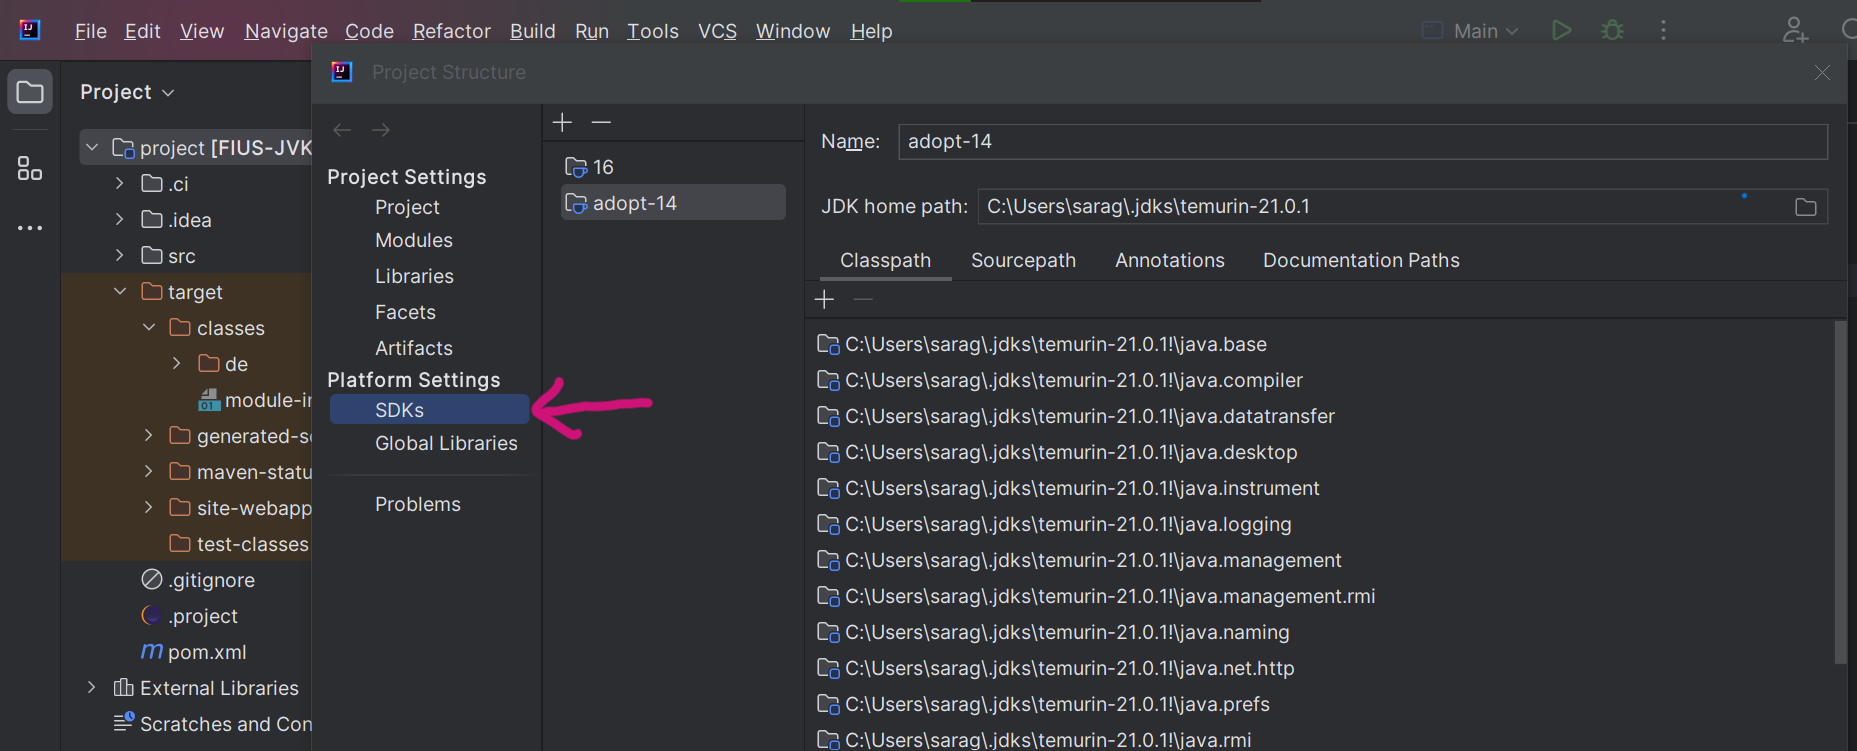
\includegraphics[width=\linewidth]{./figures/IntelliJ JDK.PNG}
\end{center}
Nun musst du entweder eine schon installierte JDK auswählen oder neue installieren. Um eine neue JDK zu installieren, musst die beiden auf Bild 2 markierten Dinge anklicken. Jetzt wird sich ein Fenster wie das in Bild 3 öffnen.
\begin{center}
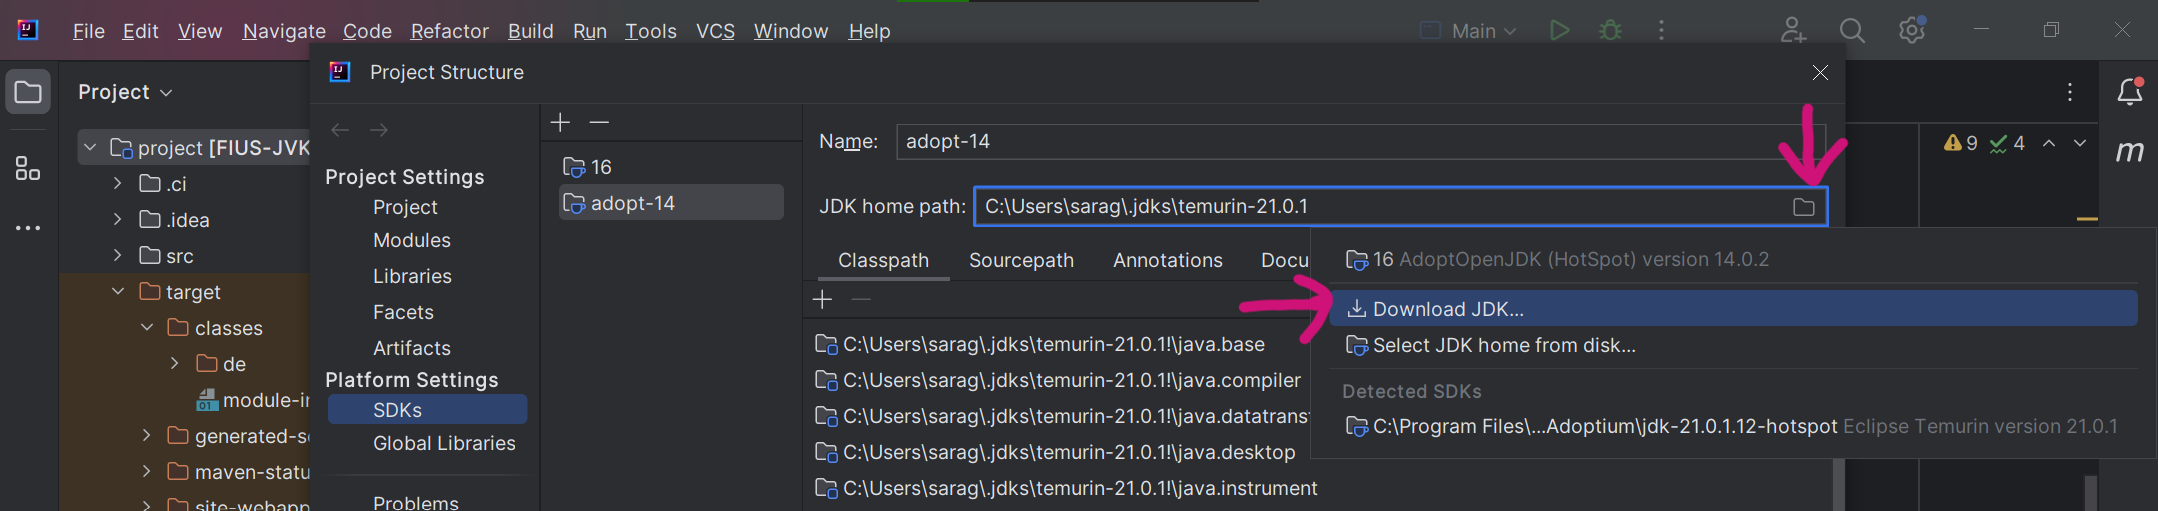
\includegraphics[width=\linewidth]{./figures/IntelliJ JDK 2.PNG}
\end{center}
\newpage
Installiere jetzt die auf dem Bild 3 gezeigte Version und füge einen sinnvollen Speicherort hinzu.
\begin{center}
    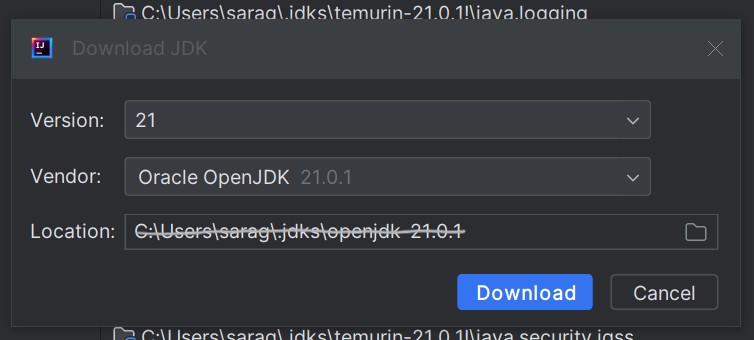
\includegraphics[width=\linewidth]{./figures/IntelliJ JDK 3.PNG}
\end{center}